\documentclass[11pt,a4paper]{article}

\usepackage[left=1.8cm,right=1.8cm,top=2.5cm,bottom=2.5cm]{geometry}
\usepackage[T1]{fontenc}
\usepackage{newtxtext,newtxmath}
\usepackage{amsmath}
\usepackage{graphicx}
\usepackage{booktabs}
\usepackage{array}
\usepackage{multirow}
\usepackage[font=small,labelfont=bf]{caption}
\usepackage{subcaption}
\usepackage[numbers,sort&compress]{natbib}
\usepackage{xcolor}
\usepackage[colorlinks=true,linkcolor=blue!50!black,citecolor=blue!50!black,urlcolor=blue!50!black]{hyperref}
\usepackage{setspace}
\setstretch{1.08}
\graphicspath{{figures/}}

\title{Does Attention Help Recurrent Models for Wearable Human Activity Recognition?\\[2pt]
\large A Subject-Independent Ablation with a Pre-Specified Decision Rule on Three Benchmarks}
\author{Himansh Munjal\\
\small [Department, Institution, City, Country]\\
\small \texttt{[corresponding-author e-mail]}}
\date{}

\begin{document}
\maketitle

\begin{abstract}
Attention modules are routinely added to recurrent networks for sensor-based human activity recognition (HAR), and reported gains are usually measured on a single random or fixed train/test split with one training run. We ask whether such gains survive a controlled, subject-independent evaluation. We build a CNN-free dual-attention bidirectional GRU whose channel attention is modulated by a new, cheap frequency-domain prior (a spectral gate computed from the low-band energy ratio and spectral entropy of each sensor channel), and evaluate it against its own ablations (no spectral gate, channel-only, temporal-only), a plain BiGRU, a BiLSTM with temporal attention, a CNN+BiGRU hybrid and DeepConvLSTM. All eight models share one training pipeline and are evaluated on UCI-HAR, WISDM and PAMAP2 with leave-subjects-out cross-validation (30 folds in total), subject-wise validation for model selection, and five seeds per fold (1{,}320 training runs). Before any of these runs existed, we fixed a decision rule: the spectral gate would be presented as a method contribution only if it beat the identical model without the gate on pooled fold-level macro-F1 (Wilcoxon signed-rank, Holm-corrected). It did not: the difference was $+0.0008$ macro-F1 (95\% CI $[-0.005, 0.007]$, $p=0.78$), and a Bayesian signed-rank test puts 99.5\% posterior probability on a practically equivalent result ($|\Delta|<0.01$). More broadly, none of the four attention variants differed from the plain BiGRU, while the two convolutional hybrids ranked best (CNN+BiGRU mean rank 3.13 of 8; pooled difference to the proposed model $-0.016$, $p_\text{Holm}=0.065$). Which subjects are held out explains 94--96\% of the variance in fold scores, whereas the choice among the eight models explains 0.4--1.5\%. Model rankings on fixed splits barely agree with the subject-independent rankings (Kendall's $\tau$ between $-0.14$ and $0.43$). We conclude that, under subject-independent evaluation, attention on top of a BiGRU does not improve wearable HAR on these benchmarks, and we give concrete recommendations for evaluating future architectural claims.
\end{abstract}

\noindent\textbf{Keywords:} human activity recognition; wearable sensors; attention; recurrent neural networks; leave-one-subject-out; statistical testing; negative results

\section{Introduction}

Human activity recognition (HAR) from wearable inertial sensors underpins applications in health monitoring, rehabilitation, sports and context-aware computing \cite{bulling2014tutorial,chen2021deep}. Deep learning replaced hand-crafted features roughly a decade ago \cite{hammerla2016deep,ordonez2016deep,ronao2016human,jiang2015human,wang2019deep}, and the field has since produced a steady stream of architectures that combine convolutional front-ends, recurrent layers and, increasingly, attention mechanisms \cite{zeng2018understanding,murahari2018attention,ma2019attnsense,gao2021danhar,pan2022gru,zhang2025dualinaba,he2025tgahar}. A popular design separates ``where to look'' (attention over sensor channels) from ``when to look'' (attention over time steps), and dual-attention recurrent models now report accuracies of 96--99\% on the standard UCI-HAR, WISDM and PAMAP2 benchmarks \cite{zhang2025dualinaba,he2025tgahar}.

How much of this progress is real is harder to say than the headline numbers suggest. Many evaluations use random or fixed train/test splits in which windows from the same person can appear on both sides, a single training run per configuration, and no statistical test; it is well documented that such protocols inflate accuracy and can reorder models \cite{hammerla2016deep,gholamiangonabadi2020deep,jordao2018human}. A recent tutorial-survey describes progress on standard HAR benchmarks as stalling \cite{haresamudram2024past}, and the broader machine-learning literature has shown that seed and data-split variance can be as large as the effects being claimed \cite{bouthillier2021accounting,lipton2019troubling}. An architectural component that adds a point of accuracy on one split may therefore add nothing under a protocol that tests generalisation to new people.

This paper reports a controlled answer to a narrow question: \emph{does attention, including a new frequency-informed variant, improve a bidirectional GRU for wearable HAR when evaluated on unseen subjects?} We started this project intending to propose a new model. To keep the conclusion from being shaped by the results, we wrote down, before the final experiment, the exact test that would justify a method claim and what the paper would be if the test failed. It failed, and this paper is the result.

\paragraph{Contributions.}
\begin{enumerate}
  \item \textbf{A spectral-gated dual-attention BiGRU (SG-DA-BiGRU).} Its channel attention is multiplied by a gate computed from two non-learned frequency descriptors of each channel (low-band energy ratio and normalised spectral entropy), at a cost of 33 parameters and one FFT per window (Section~\ref{sec:method}).
  \item \textbf{A controlled ablation and baseline study.} Eight models, including the published DeepConvLSTM configuration \cite{ordonez2016deep}, are trained with one shared pipeline on three benchmarks using subject-independent cross-validation with subject-wise validation, five seeds per fold and 1{,}320 runs in total (Section~\ref{sec:protocol}).
  \item \textbf{A pre-specified decision rule and its outcome.} The spectral gate does not improve on the identical model without it, and the evidence supports practical equivalence rather than merely an inconclusive result. None of the attention variants differs from a plain BiGRU (Section~\ref{sec:results}).
  \item \textbf{An analysis of evaluation itself.} We quantify how much fold-to-fold (subject) variance dominates model differences, show that fixed-split rankings are unreliable proxies for subject-independent rankings, and document how selecting checkpoints on validation loss rather than validation macro-F1 caused premature stopping in our first protocol (Sections~\ref{sec:protocolfix}, \ref{sec:variance} and \ref{sec:fixed}).
  \item \textbf{Practical recommendations} for evaluating architectural claims in wearable HAR (Section~\ref{sec:discussion}). Code, configurations, per-run results and predictions are released.
\end{enumerate}

\section{Related Work}
\label{sec:related}

\paragraph{Deep models for wearable HAR.}
Early deep HAR work showed that convolutional networks learn useful local motion features from raw inertial signals \cite{jiang2015human,ronao2016human}, and that recurrent networks capture longer temporal context \cite{hammerla2016deep,guan2017ensembles}. DeepConvLSTM \cite{ordonez2016deep}, four temporal convolutions followed by two LSTM layers, became the reference architecture, and convolutional-recurrent hybrids remain the dominant family \cite{xia2020lstm,mutegeki2020cnn}. Several studies show that simpler variants can match or beat deeper ones: Bock et al.\ \cite{bock2021improving} improved DeepConvLSTM by \emph{removing} an LSTM layer, and Hammerla et al.\ \cite{hammerla2016deep} found that hyper-parameter choices often matter more than architecture. Surveys \cite{wang2019deep,chen2021deep,haresamudram2024past} give broad overviews; self-supervised pre-training is an active alternative direction \cite{tang2021selfhar,haresamudram2022assessing}.

\paragraph{Attention for sensor-based HAR.}
Attention was introduced to sequence models as a learned weighting of hidden states \cite{bahdanau2015neural} and generalised by the Transformer \cite{vaswani2017attention}. In computer vision, squeeze-and-excitation \cite{hu2018squeeze} and CBAM \cite{woo2018cbam} popularised channel attention computed from pooled feature statistics. In HAR, Zeng et al.\ \cite{zeng2018understanding} added temporal and sensor attention to LSTMs; Murahari and Pl\"otz \cite{murahari2018attention} added temporal attention to DeepConvLSTM; AttnSense \cite{ma2019attnsense} combined attention across sensor modalities and time; DanHAR \cite{gao2021danhar} combined channel and temporal attention on a CNN; and Pan et al.\ \cite{pan2022gru} proposed a GRU with dual (channel and temporal) attention. Recent hybrids add Inception or temporal-convolution branches to attention-augmented BiGRUs, e.g.\ Dual-INABA \cite{zhang2025dualinaba} on UCI-HAR, WISDM and PAMAP2 and TGA-HAR \cite{he2025tgahar} on WISDM, USC-HAD and PAMAP2. To our knowledge, these models compute channel attention only from learned time-domain statistics; none injects an explicit frequency-domain prior, which is the gap our spectral gate targets. Whether attention weights are informative is itself debated \cite{jain2019attention,serrano2019attention}; we do not rely on attention for interpretation.

\paragraph{Evaluation practice.}
Windows from one recording overlap strongly, so random window-level splits leak subject identity into the test set; leave-one-subject-out (LOSO) cross-validation gives lower but more honest estimates and changes which model is selected \cite{gholamiangonabadi2020deep,jordao2018human,hammerla2016deep}. For comparing models across folds or data sets, Dem\v{s}ar \cite{demsar2006statistical} recommends non-parametric tests (Wilcoxon signed-rank \cite{wilcoxon1945individual}, Friedman \cite{friedman1937use}) with multiple-comparison control \cite{holm1979simple}; Benavoli et al.\ argue against mean-rank post-hoc tests for pairwise claims \cite{benavoli2016should} and advocate Bayesian tests with a region of practical equivalence \cite{benavoli2017time}. Bouthillier et al.\ \cite{bouthillier2021accounting} show that ignoring seed and data-split variance yields unreliable conclusions. The recent dual-attention HAR models above report accuracy on a single split without significance tests or computational cost; this study supplies the missing controlled comparison for this model family.

\section{Models}
\label{sec:method}

Each input is a window $x\in\mathbb{R}^{T\times C}$ of $T$ time steps and $C$ sensor channels, z-scored per channel with statistics from the training subjects of the current fold. The task is to predict one of $K$ activity classes.

\subsection{Spectral-gated dual-attention BiGRU}
Figure~\ref{fig:arch} shows the proposed model.

\paragraph{Learned channel attention.}
Following CBAM \cite{woo2018cbam}, each channel is summarised by its temporal mean and maximum, and a shared bottleneck MLP ($C\to\max(1,\lfloor C/4\rfloor)\to C$) produces independent per-channel gates
\begin{equation}
a = \sigma\big(\mathrm{MLP}(\operatorname{mean}_t x) + \mathrm{MLP}(\operatorname{max}_t x)\big)\in(0,1)^C .
\end{equation}
Sigmoid rather than softmax gates are used so that several channels can be important at once.

\paragraph{Spectral gate.}
For each channel $c$ we compute the power spectrum $P_f=|\mathrm{rFFT}(x_{:,c})|^2$, $f=1,\dots,F$, and two descriptors:
\begin{equation}
\rho_c = \frac{\sum_{f\in\mathcal{B}} P_f}{\sum_{f} P_f},\qquad
H_c = -\frac{1}{\log F}\sum_f p_f\log p_f,\quad p_f = \frac{P_f}{\sum_{f'}P_{f'}},
\end{equation}
where $\mathcal{B}$ is the 0.3--3.5\,Hz band in physical units (using each data set's sampling rate), which covers gait and limb-swing frequencies. $\rho_c$ is high for channels dominated by periodic locomotion and low for near-static channels, and $H_c$ is low for clean periodic signals and high for broadband noise. A tiny MLP shared across channels ($2\to8\to1$, tanh) maps $(\rho_c,H_c)$ to a gate $g_c=\sigma(\cdot)$. It has 33 parameters and needs no learned transform before it. The intended inductive bias is that a time-domain attention MLP cannot easily measure periodicity from a single window, whereas the FFT gives it directly.

\paragraph{Reweighting, recurrence and temporal attention.}
The two gates are combined and renormalised so that the average channel weight stays at one, i.e.\ the gate does not change the overall input scale:
\begin{equation}
w = \frac{a\odot g}{\tfrac{1}{C}\sum_c a_c g_c+\epsilon},\qquad \tilde{x}_{t,c}=w_c\,x_{t,c}.
\end{equation}
$\tilde{x}$ is processed by a two-layer bidirectional GRU \cite{cho2014learning,schuster1997bidirectional} with 64 units per direction and dropout 0.3 between layers \cite{srivastava2014dropout}, giving states $h_t\in\mathbb{R}^{128}$. Additive temporal attention \cite{bahdanau2015neural} pools them:
\begin{equation}
\alpha_t=\operatorname{softmax}_t\big(v^\top\tanh(W h_t+b)\big),\qquad z=\sum_t\alpha_t h_t ,
\end{equation}
with a 64-dimensional attention layer. A head (FC 128, ReLU, dropout 0.3, FC $K$) produces logits.

\begin{figure}[!htbp]
  \centering
  \begin{subfigure}[b]{0.56\linewidth}
    \centering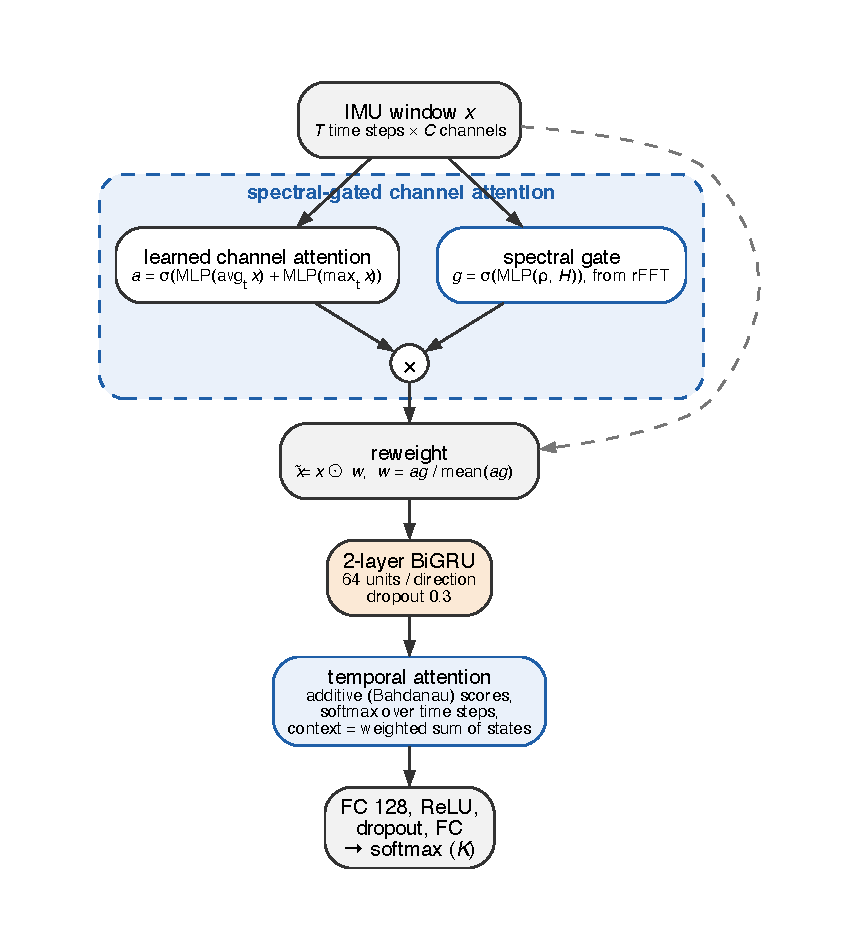
\includegraphics[width=\linewidth]{fig_arch}
    \caption{SG-DA-BiGRU. The dashed edge carries the unweighted input $x$ to the reweighting step.}
  \end{subfigure}\hfill
  \begin{subfigure}[b]{0.40\linewidth}
    \centering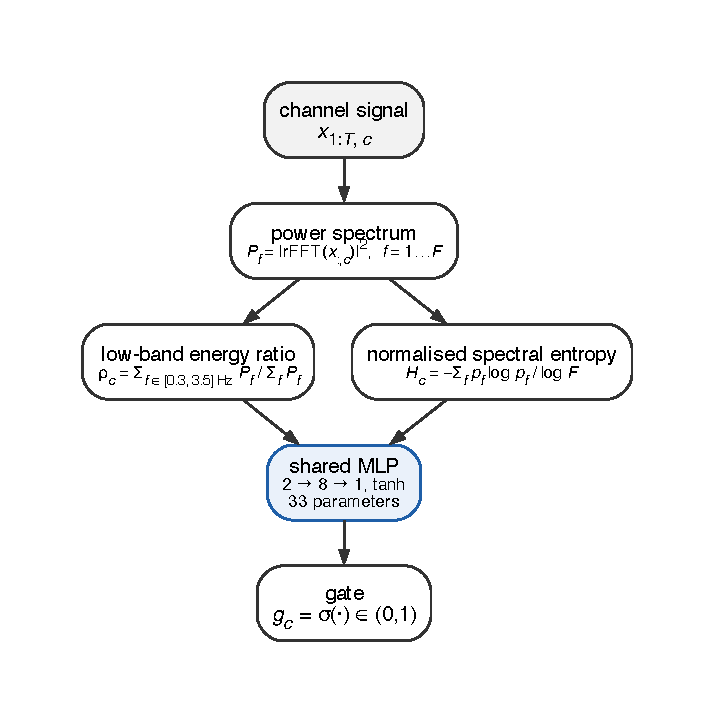
\includegraphics[width=\linewidth]{fig_gate}
    \caption{Spectral gate for one channel $c$; the MLP is shared across channels.}
  \end{subfigure}
  \caption{Architecture of the proposed spectral-gated dual-attention BiGRU. Blue outlines mark the components removed in the ablations (Table~\ref{tab:arms}).}
  \label{fig:arch}
\end{figure}

\subsection{Ablations and baselines}
Table~\ref{tab:arms} lists the eight models. The four dual-attention arms share the same code and differ only by switching components on or off. \emph{DA-BiGRU} (``plain'') removes the spectral gate, and corresponds to the learned channel + temporal dual attention used in prior work \cite{pan2022gru,zhang2025dualinaba}. The full-versus-plain contrast therefore isolates the spectral gate. \emph{Channel-only} keeps the spectral-gated channel attention but replaces temporal attention with mean pooling. \emph{Temporal-only} drops channel attention.

The baselines are a plain two-layer BiGRU with mean pooling, a two-layer BiLSTM \cite{hochreiter1997long} with the same additive temporal attention, a CNN+BiGRU hybrid (three Conv1D blocks with 64/128/128 filters, kernel sizes 5/5/3, batch norm, two max-pooling stages, then the same BiGRU), and DeepConvLSTM in its published configuration \cite{ordonez2016deep}: four $5\times1$ convolutions with 64 filters, two 128-unit LSTM layers with dropout 0.5, and classification from the last time step. All models except DeepConvLSTM use the same hidden size, depth, dropout and head. Two-layer recurrent networks are built as stacks of single-layer cuDNN RNNs with dropout between them, which is mathematically identical to the fused multi-layer RNN.

\begin{table}[!htbp]
\centering
\caption{The eight compared models. ``mean-pool'' means temporal attention is replaced by averaging the recurrent states over time.}
\label{tab:arms}
\small
\setlength{\tabcolsep}{4pt}
\begin{tabular}{llcccl}
\toprule
Model & Backbone & Channel attn. & Spectral gate & Temporal attn. & Front-end \\
\midrule
SG-DA-BiGRU (proposed, ``full'') & BiGRU & \checkmark & \checkmark & \checkmark & none \\
DA-BiGRU (``plain'') & BiGRU & \checkmark & -- & \checkmark & none \\
Channel-only & BiGRU & \checkmark & \checkmark & mean-pool & none \\
Temporal-only & BiGRU & -- & -- & \checkmark & none \\
\midrule
BiGRU & BiGRU & -- & -- & mean-pool & none \\
BiLSTM+Attn & BiLSTM & -- & -- & \checkmark & none \\
CNN+BiGRU & BiGRU & -- & -- & mean-pool & 3$\times$Conv1D \\
DeepConvLSTM \cite{ordonez2016deep} & LSTM (uni.) & -- & -- & last step & 4$\times$Conv \\
\bottomrule
\end{tabular}
\end{table}

\section{Experimental Protocol}
\label{sec:protocol}

\subsection{Data sets and preprocessing}
Table~\ref{tab:data} summarises the three benchmarks. \textbf{UCI-HAR} \cite{anguita2013public} contains 30 subjects with a waist-mounted smartphone; we use the source's 2.56\,s windows (128 samples at 50\,Hz, 50\% overlap) and six channels (total acceleration and gyroscope, three axes each). \textbf{WISDM} v1.1 \cite{kwapisz2011activity} contains 36 subjects with a pocket smartphone accelerometer at 20\,Hz; we keep the file's recording order and cut 51-sample windows (about 2.56\,s) with a 25-sample step, discarding windows that cross a subject or activity boundary. \textbf{PAMAP2} \cite{reiss2012introducing} (protocol activities) contains three IMUs (hand, chest, ankle); we use the $\pm16g$ accelerometer and gyroscope of each IMU (18 channels), linearly interpolate sensor dropouts, downsample from 100 to 50\,Hz with an anti-aliasing polyphase filter, and cut 128-sample windows with 50\% overlap. Subject 109, who recorded almost no protocol activities, is excluded, leaving eight subjects and 12 classes. Windows are labelled only if every sample in them carries the same label.

\begin{table}[!htbp]
\centering
\caption{Benchmarks and evaluation folds. All data sets use 2.56\,s windows with 50\% overlap. The fixed split is the official 21/9-subject split for UCI-HAR and a seeded subject-level 80/20 split for WISDM and PAMAP2, which publish no official split.}
\label{tab:data}
\small
\begin{tabular}{lcccccccc}
\toprule
Data set & Subjects & Classes & Channels & Rate & $T$ & Windows & LOSO folds & Test subj./fold \\
\midrule
UCI-HAR \cite{anguita2013public} & 30 & 6 & 6 & 50\,Hz & 128 & 10{,}299 & 10 & 3 \\
WISDM \cite{kwapisz2011activity} & 36 & 6 & 3 & 20\,Hz & 51 & 42{,}657 & 12 & 3 \\
PAMAP2 \cite{reiss2012introducing} & 8 & 12 & 18 & 50\,Hz & 128 & 14{,}922 & 8 & 1 \\
\bottomrule
\end{tabular}
\end{table}

\subsection{Subject-independent evaluation}
The primary protocol is leave-subjects-out cross-validation (Figure~\ref{fig:protocol}). Subjects are shuffled once with a fixed seed and partitioned into 10 (UCI-HAR), 12 (WISDM) or 8 (PAMAP2, i.e.\ true LOSO) folds, giving 30 test folds in total. Within each fold, 20\% of the training subjects (at least two) form a \emph{subject-wise} validation set used for early stopping and learning-rate scheduling, so test subjects never influence training or model selection. Normalisation statistics are fitted on the remaining training subjects only. Every model is trained with five seeds (0--4) on every fold, and the fold score is the mean over seeds; seeds on the same fold are not independent and are never treated as separate samples. We also report the fixed train/test split described in Table~\ref{tab:data}, with five seeds, as a secondary analysis.

\begin{figure}[!htbp]
  \centering
  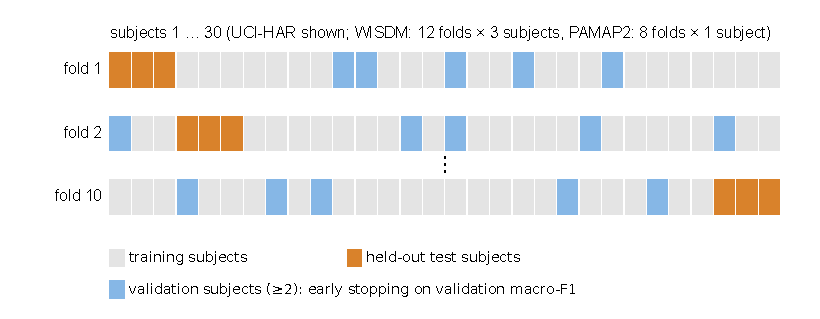
\includegraphics[width=0.95\linewidth]{fig_protocol}
  \caption{Subject-independent protocol (schematic; subject assignment to folds is shuffled with a fixed seed). In every fold the test subjects are unseen, and model selection uses separate validation subjects.}
  \label{fig:protocol}
\end{figure}

\subsection{Training}
All models are trained with Adam \cite{kingma2015adam} (learning rate $10^{-3}$, batch size 64, cross-entropy loss) for at most 50 epochs, with gradient-norm clipping at 1.0, ReduceLROnPlateau (factor 0.5, patience 3) and early stopping (patience 8). Both the scheduler and early stopping monitor validation macro-F1, and the checkpoint with the best validation macro-F1 is restored before testing. No model received individual hyper-parameter tuning, so every model was trained under the same budget and rules. Training used PyTorch \cite{paszke2019pytorch} with deterministic cuDNN on one NVIDIA GeForce RTX 3050 Laptop GPU (4\,GB). The 1{,}320 runs took 27.6 GPU-hours of training time in total.

\subsection{Metrics and statistical analysis}
The primary metric is macro-F1, the unweighted mean of per-class F1, which is robust to class imbalance; we also report accuracy. Following scikit-learn's default, macro-F1 is averaged over every class that occurs in the labels or predictions of a fold, so false positives of a class absent from a test subject count as an F1 of zero. This lowers absolute PAMAP2 scores, where not every subject performed every activity, but affects all models equally.

\paragraph{Pre-specified decision rule.}
The rule below was written into the project's protocol document and committed to the repository on 2026-10-16, before any run of the final protocol existed. \emph{Primary endpoint:} LOSO macro-F1, one value per fold (mean over seeds), pooled over the three data sets (30 folds); two-sided Wilcoxon signed-rank test \cite{wilcoxon1945individual}, Holm-corrected \cite{holm1979simple} over the seven comparisons of SG-DA-BiGRU against every other model. The paper would be framed as a method contribution only if (i) SG-DA-BiGRU beat DA-BiGRU on this endpoint with $p_\text{Holm}<0.05$, and (ii) SG-DA-BiGRU was not significantly worse than any baseline. Otherwise it would be an empirical study. Per-data-set tests and the fixed splits are secondary. The smallest attainable two-sided Wilcoxon $p$ is 0.002 with 10 folds, $5\times10^{-4}$ with 12, 0.008 with 8 (0.055 after Holm, so PAMAP2 alone cannot reach significance) and $<10^{-8}$ with 30.

\paragraph{Supporting analyses.}
We report 95\% bootstrap confidence intervals of the mean fold difference (10{,}000 resamples), the Friedman test \cite{friedman1937use} with the Iman--Davenport correction and Nemenyi critical-difference diagram over all eight models \cite{demsar2006statistical}, and the Bayesian signed-rank test \cite{benavoli2017time} with a region of practical equivalence (ROPE) of $\pm0.01$ macro-F1 and a prior strength of $0.5$. These analyses were added after the decision rule was fixed and are descriptive.

\subsection{Computational cost}
Parameters are counted exactly. FLOPs per window are multiply--accumulate counts from the \texttt{thop} profiler, which approximates recurrent layers and does not count FFT operations, so the spectral gate's cost shows up in latency but not in FLOPs. Inference latency was measured in a separate, controlled pass (median of 100 forward passes after 20 warm-up passes) on the same laptop GPU and on one CPU thread, at batch sizes 1 and 32.

\subsection{Protocol revision before the final run}
\label{sec:protocolfix}
For transparency, we report that the protocol above is the second version. A first full run (483 runs; 6/6/8 folds; three seeds; one validation subject on PAMAP2; checkpoint selection on validation \emph{loss}) showed that under subject shift the validation loss rises after one to three epochs while validation macro-F1 keeps improving: 43.5\% of runs selected an epoch $\le3$ (Figure~\ref{fig:epochs}). We diagnosed this from the training curves, not from which model won, and changed the protocol identically for all models: selection on validation macro-F1, at least two validation subjects, more folds and seeds, and DeepConvLSTM added as a fourth baseline. The decision rule was fixed at the same time. After the change, the median selected epoch rose from 4 to 9 and the share of runs stopping by epoch 3 fell to 13.3\%; 11 of 1{,}320 runs reached the 50-epoch limit. The first run gave the same answer to the primary question (spectral gate vs.\ none: $+0.003$ macro-F1 over 20 folds, $p=0.73$). All numbers below come from the final protocol.

\begin{figure}[!htbp]
  \centering
  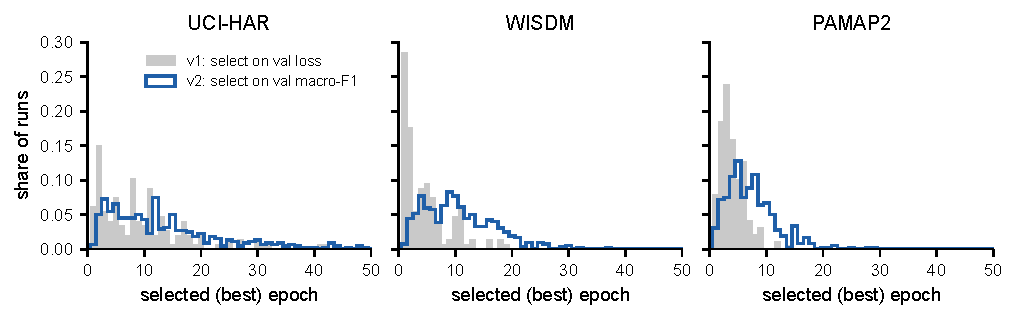
\includegraphics[width=\linewidth]{fig_epochs}
  \caption{Selected (best) epoch per run when checkpoints are chosen by validation loss (first protocol, grey, 483 runs) versus validation macro-F1 (final protocol, blue, 1{,}320 runs).}
  \label{fig:epochs}
\end{figure}

\section{Results}
\label{sec:results}

\subsection{Subject-independent performance}
Table~\ref{tab:loso} and Figure~\ref{fig:loso} report LOSO macro-F1. On UCI-HAR all eight models fall within 0.009 of each other (0.916--0.925). On WISDM, CNN+BiGRU is highest (0.838) and the attention variants range from 0.805 to 0.820. On PAMAP2, DeepConvLSTM is highest (0.746) and the recurrent models without convolutions reach 0.674--0.697. Pooled over the 30 folds, the two convolutional hybrids lead (0.832 each), followed by BiLSTM+Attn (0.819), the plain BiGRU (0.816) and the four dual-attention variants (0.813--0.815). Accuracy (Table~\ref{tab:acc}) gives the same picture. Standard deviations across folds (0.04--0.21) are an order of magnitude larger than the gaps between models, which is the subject of Section~\ref{sec:variance}.

\begin{table}[!htbp]
\centering
\caption{Subject-independent (LOSO) macro-F1, mean $\pm$ standard deviation across folds (each fold averaged over five seeds). Bold marks the best model per column.}
\label{tab:loso}
\small
\begin{tabular}{lcccc}
\toprule
Model & UCI-HAR (10 folds) & WISDM (12) & PAMAP2 (8) & Pooled (30) \\
\midrule
BiGRU & 0.920 $\pm$ 0.049 & 0.810 $\pm$ 0.094 & 0.695 $\pm$ 0.198 & 0.816 $\pm$ 0.146 \\
BiLSTM+Attn & 0.921 $\pm$ 0.049 & 0.820 $\pm$ 0.091 & 0.687 $\pm$ 0.185 & 0.819 $\pm$ 0.143 \\
CNN+BiGRU & \textbf{0.925} $\pm$ 0.042 & \textbf{0.838} $\pm$ 0.091 & 0.705 $\pm$ 0.207 & 0.832 $\pm$ 0.147 \\
DeepConvLSTM & 0.917 $\pm$ 0.051 & 0.820 $\pm$ 0.085 & \textbf{0.746} $\pm$ 0.109 & \textbf{0.832} $\pm$ 0.105 \\
\midrule
SG-DA-BiGRU & 0.922 $\pm$ 0.045 & 0.813 $\pm$ 0.091 & 0.685 $\pm$ 0.190 & 0.815 $\pm$ 0.145 \\
DA-BiGRU & 0.921 $\pm$ 0.047 & 0.820 $\pm$ 0.087 & 0.674 $\pm$ 0.191 & 0.815 $\pm$ 0.148 \\
Channel-only & 0.916 $\pm$ 0.051 & 0.805 $\pm$ 0.093 & 0.697 $\pm$ 0.184 & 0.813 $\pm$ 0.140 \\
Temporal-only & 0.918 $\pm$ 0.053 & 0.816 $\pm$ 0.089 & 0.678 $\pm$ 0.178 & 0.813 $\pm$ 0.143 \\
\bottomrule
\end{tabular}
\end{table}

\begin{figure}[!htbp]
  \centering
  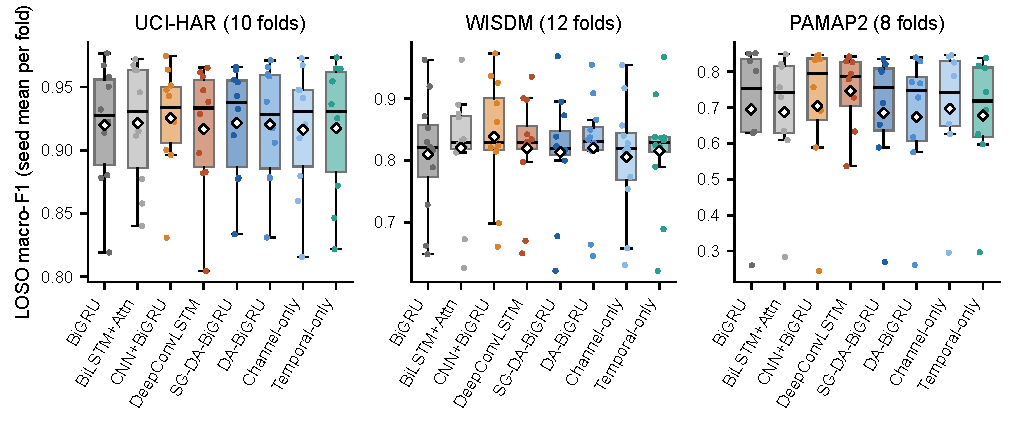
\includegraphics[width=\linewidth]{fig_loso}
  \caption{LOSO macro-F1 per fold (dots; mean over five seeds), with box plots and means (diamonds). Differences between models are small compared with the spread across folds.}
  \label{fig:loso}
\end{figure}

\subsection{Primary endpoint: does the spectral gate help?}
\label{sec:primary}
Table~\ref{tab:sig} gives the pre-specified tests. SG-DA-BiGRU and DA-BiGRU differ by $+0.0008$ macro-F1 (95\% CI $[-0.0051, +0.0067]$); the gate wins on 17 of 30 folds, $p=0.777$, $p_\text{Holm}=1.0$. \textbf{Condition (i) of the decision rule fails, so this paper is an empirical study, not a method paper.} Condition (ii) holds, but narrowly: CNN+BiGRU is better than the proposed model by 0.016 (CI $[-0.029, -0.004]$, 21 of 30 folds), with raw $p=0.009$ and $p_\text{Holm}=0.065$.

\begin{table}[!htbp]
\centering
\caption{Pre-specified primary analysis: SG-DA-BiGRU minus each comparator, LOSO macro-F1 pooled over 30 folds. Wins: folds on which SG-DA-BiGRU is better. $p$: two-sided Wilcoxon signed-rank; $p_\text{Holm}$: Holm-corrected over the seven comparisons.}
\label{tab:sig}
\small
\begin{tabular}{lccccc}
\toprule
Comparator & $\Delta$ macro-F1 & 95\% bootstrap CI & Wins & $p$ & $p_\text{Holm}$ \\
\midrule
BiGRU & -0.0006 & [-0.0096, +0.0098] & 13/30 & 0.584 & 1.000 \\
BiLSTM+Attn & -0.0031 & [-0.0095, +0.0032] & 11/30 & 0.253 & 1.000 \\
CNN+BiGRU & -0.0164 & [-0.0293, -0.0040] & 9/30 & 0.009 & 0.065 \\
DeepConvLSTM & -0.0171 & [-0.0404, +0.0005] & 11/30 & 0.184 & 1.000 \\
DA-BiGRU & +0.0008 & [-0.0051, +0.0067] & 17/30 & 0.777 & 1.000 \\
Channel-only & +0.0020 & [-0.0077, +0.0125] & 16/30 & 0.792 & 1.000 \\
Temporal-only & +0.0025 & [-0.0040, +0.0095] & 16/30 & 0.777 & 1.000 \\
\bottomrule
\end{tabular}
\end{table}

A non-significant test alone does not show that the gate has no effect. Two further analyses show that the effect is small, not merely uncertain. The Bayesian signed-rank test (Table~\ref{tab:bayes}) gives a posterior probability of 0.995 that the full-versus-plain difference lies within $\pm0.01$ macro-F1. The Bayesian bootstrap of the mean difference (Figure~\ref{fig:fvp}b) places 99.8\% of its mass in the same interval, with a 95\% interval of $[-0.005, +0.007]$. Per fold, the two models track each other closely across the whole range of difficulty (Figure~\ref{fig:fvp}a). The same holds for the attention components more generally: SG-DA-BiGRU is practically equivalent to the plain BiGRU (posterior 0.80), BiLSTM+Attn (0.97) and Temporal-only (0.96). In contrast, the posterior probability that it is worse than CNN+BiGRU is 0.95.

\begin{table}[!htbp]
\centering
\caption{Bayesian signed-rank test \cite{benavoli2017time} on the 30 pooled folds (ROPE $\pm0.01$ macro-F1): posterior probability that SG-DA-BiGRU is better than, practically equivalent to, or worse than each comparator.}
\label{tab:bayes}
\small
\begin{tabular}{lccc}
\toprule
Comparator & $P(\text{better})$ & $P(\text{equivalent})$ & $P(\text{worse})$ \\
\midrule
BiGRU & 0.030 & 0.804 & 0.166 \\
BiLSTM+Attn & 0.001 & 0.973 & 0.025 \\
CNN+BiGRU & 0.003 & 0.043 & 0.954 \\
DeepConvLSTM & 0.027 & 0.322 & 0.652 \\
DA-BiGRU & 0.004 & 0.995 & 0.001 \\
Channel-only & 0.106 & 0.850 & 0.044 \\
Temporal-only & 0.039 & 0.959 & 0.003 \\
\bottomrule
\end{tabular}
\end{table}

\begin{figure}[!htbp]
  \centering
  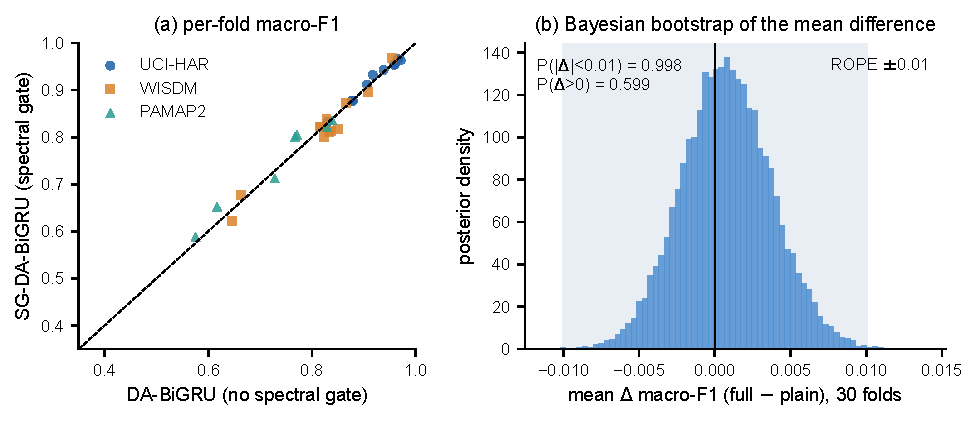
\includegraphics[width=\linewidth]{fig_full_vs_plain}
  \caption{The pre-specified contrast. (a) Per-fold macro-F1 with and without the spectral gate; points lie on the diagonal. (b) Bayesian-bootstrap posterior of the mean difference over 30 folds; the shaded band is the region of practical equivalence ($\pm0.01$).}
  \label{fig:fvp}
\end{figure}

\subsection{Per-data-set comparisons}
Figure~\ref{fig:forest} and Table~\ref{tab:sigds} break the comparisons down by data set. No per-data-set difference survives Holm correction. The two largest are WISDM, where CNN+BiGRU beats SG-DA-BiGRU on 11 of 12 folds ($\Delta=-0.025$, raw $p=0.021$, $p_\text{Holm}=0.147$), and PAMAP2, where DeepConvLSTM is ahead by 0.061 but, with eight folds, cannot reach significance. Within the attention family, the sign of the full-versus-plain difference flips between data sets ($+0.001$, $-0.007$, $+0.012$), which is what one expects from noise around zero.

\begin{figure}[!htbp]
  \centering
  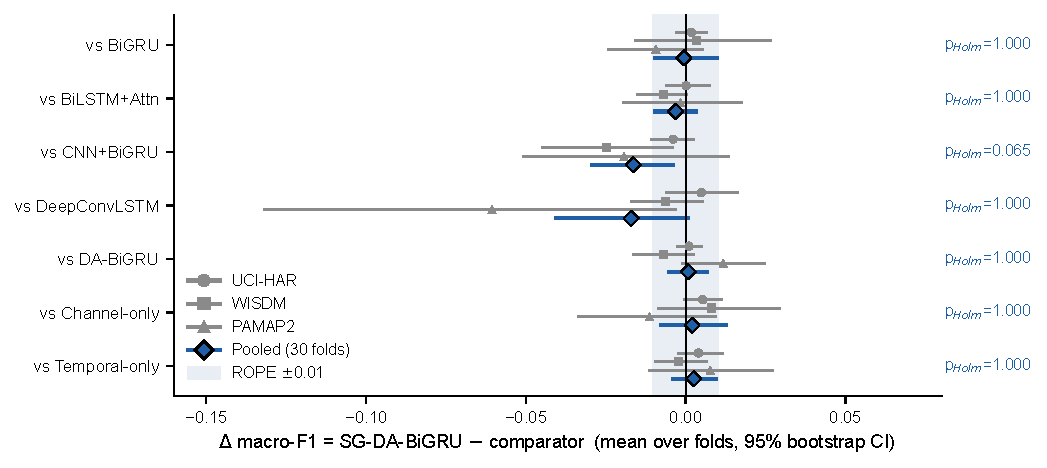
\includegraphics[width=\linewidth]{fig_forest}
  \caption{Mean fold-level difference in macro-F1 (SG-DA-BiGRU minus comparator) with 95\% bootstrap confidence intervals, per data set (grey) and pooled (blue). The shaded band is the $\pm0.01$ region of practical equivalence; Holm-corrected pooled $p$-values are shown on the right.}
  \label{fig:forest}
\end{figure}

\begin{table}[!htbp]
\centering
\caption{Per-data-set comparisons (secondary): mean difference SG-DA-BiGRU minus comparator, folds won, and Holm-corrected Wilcoxon $p$ within each data set.}
\label{tab:sigds}
\small
\setlength{\tabcolsep}{4.5pt}
\begin{tabular}{lccccccccc}
\toprule
& \multicolumn{3}{c}{UCI-HAR (10 folds)} & \multicolumn{3}{c}{WISDM (12 folds)} & \multicolumn{3}{c}{PAMAP2 (8 folds)} \\
\cmidrule(lr){2-4}\cmidrule(lr){5-7}\cmidrule(lr){8-10}
Comparator & $\Delta$ & Wins & $p_\text{Holm}$ & $\Delta$ & Wins & $p_\text{Holm}$ & $\Delta$ & Wins & $p_\text{Holm}$ \\
\midrule
BiGRU & +0.0018 & 4/10 & 1.000 & +0.0034 & 6/12 & 1.000 & -0.0093 & 3/8 & 1.000 \\
BiLSTM+Attn & +0.0001 & 3/10 & 1.000 & -0.0069 & 5/12 & 1.000 & -0.0016 & 3/8 & 1.000 \\
CNN+BiGRU & -0.0039 & 5/10 & 1.000 & -0.0249 & 1/12 & 0.147 & -0.0193 & 3/8 & 1.000 \\
DeepConvLSTM & +0.0049 & 5/10 & 1.000 & -0.0063 & 4/12 & 1.000 & -0.0606 & 2/8 & 1.000 \\
DA-BiGRU & +0.0010 & 6/10 & 1.000 & -0.0068 & 6/12 & 1.000 & +0.0118 & 5/8 & 1.000 \\
Channel-only & +0.0053 & 6/10 & 1.000 & +0.0081 & 6/12 & 1.000 & -0.0113 & 4/8 & 1.000 \\
Temporal-only & +0.0040 & 6/10 & 1.000 & -0.0023 & 5/12 & 1.000 & +0.0077 & 5/8 & 1.000 \\
\bottomrule
\end{tabular}
\end{table}

\subsection{Ranking all eight models}
The Friedman test over 30 folds rejects equal performance of the eight models ($\chi^2_7=15.67$, $p=0.028$; Iman--Davenport $F_{7,203}=2.34$, $p=0.026$). The critical-difference diagram (Figure~\ref{fig:cd}) orders the models CNN+BiGRU (mean rank 3.13), DeepConvLSTM (4.13), BiLSTM+Attn (4.23), BiGRU (4.50), SG-DA-BiGRU and DA-BiGRU (4.90 each), Temporal-only (5.00) and Channel-only (5.20). With $\mathrm{CD}=1.92$, only CNN+BiGRU versus Channel-only exceeds the critical difference. The four dual-attention variants occupy the bottom four ranks, though within a band narrower than the critical difference. As \cite{benavoli2016should} cautions, mean-rank post-hoc tests depend on which other models are included; we therefore base pairwise claims on Tables~\ref{tab:sig}--\ref{tab:bayes} and use the ranking only descriptively.

\begin{figure}[!htbp]
  \centering
  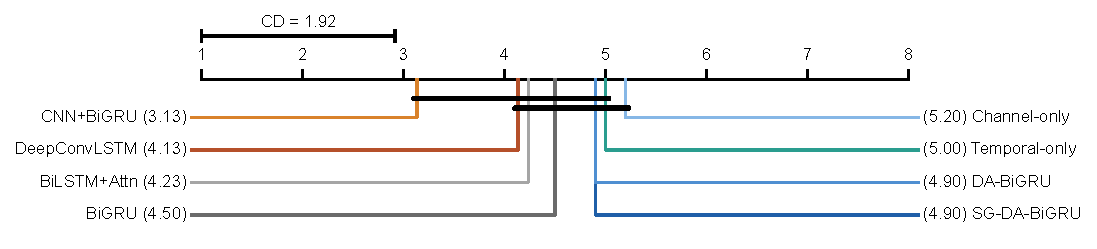
\includegraphics[width=0.95\linewidth]{fig_cd}
  \caption{Mean rank of each model across the 30 LOSO folds (1 = best). Models joined by a bar are not separated by the Nemenyi critical difference ($\alpha=0.05$).}
  \label{fig:cd}
\end{figure}

\subsection{Where the convolutional front-end helps}
Figure~\ref{fig:perclass} shows per-class F1 relative to the plain BiGRU, computed from the pooled LOSO predictions and averaged over seeds. On UCI-HAR all models agree to within about two points per class. On WISDM, CNN+BiGRU improves the two hardest classes, walking upstairs (+5.3 points) and downstairs (+3.7), as well as sitting (+3.5) and standing (+3.4); SG-DA-BiGRU and DA-BiGRU mainly improve sitting (+8 and +7). On PAMAP2, DeepConvLSTM is better on most classes, notably walking (+10.2), ironing (+7.9), vacuuming (+6.9) and sitting (+5.5). In contrast, SG-DA-BiGRU loses 9.8 points on ascending stairs. So the convolutional front-ends help most where short, local motion patterns separate similar activities (stairs vs.\ walking, postural differences among low-motion household tasks). That is the kind of information a learned time-domain filter extracts and a per-channel gain does not.

\begin{figure}[!htbp]
  \centering
  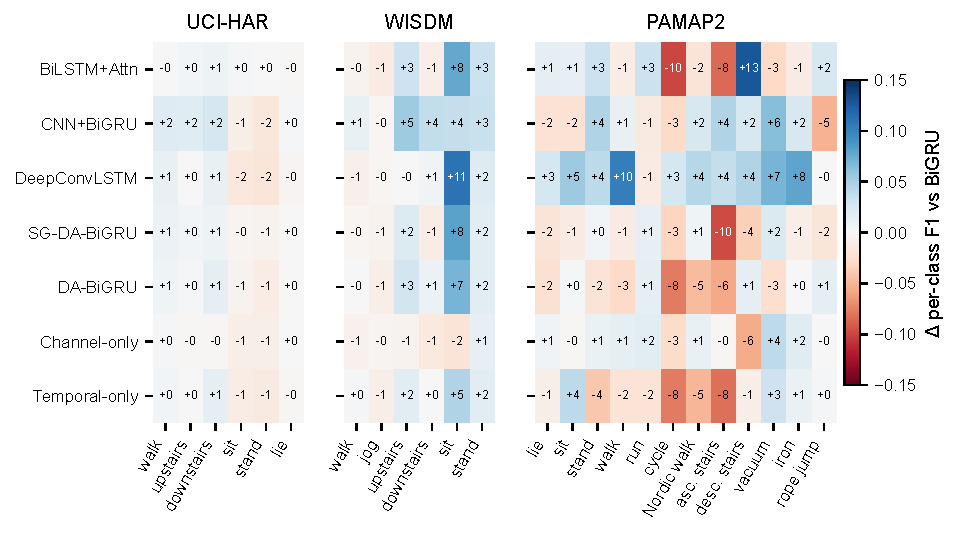
\includegraphics[width=\linewidth]{fig_perclass}
  \caption{Per-class F1 difference to the plain BiGRU (percentage points), LOSO predictions pooled over folds and averaged over seeds.}
  \label{fig:perclass}
\end{figure}

\subsection{Subjects, not architectures, dominate the variance}
\label{sec:variance}
Figure~\ref{fig:variance}a compares three sources of variation in macro-F1. Seed-to-seed standard deviation within a fold is 0.014 (UCI-HAR), 0.025 (WISDM) and 0.048 (PAMAP2). Fold-to-fold standard deviation is 3.4--3.8 times larger (0.048, 0.090, 0.180), and the spread of the eight model means is 0.003, 0.010 and 0.023. In a two-way decomposition of the seed-averaged fold scores, the fold factor explains 96.2\%, 93.8\% and 94.3\% of the variance on the three data sets, and the model factor only 0.4\%, 1.1\% and 1.5\%. Per held-out subject (Figure~\ref{fig:variance}b), the proposed model's macro-F1 ranges from 0.64 to 1.00 on UCI-HAR, from 0.16 to 0.97 on WISDM and from 0.27 to 0.84 on PAMAP2. Who is in the test set therefore matters far more than which of these architectures is used, and a fixed split with a single seed has no chance of separating the models.

\begin{figure}[!htbp]
  \centering
  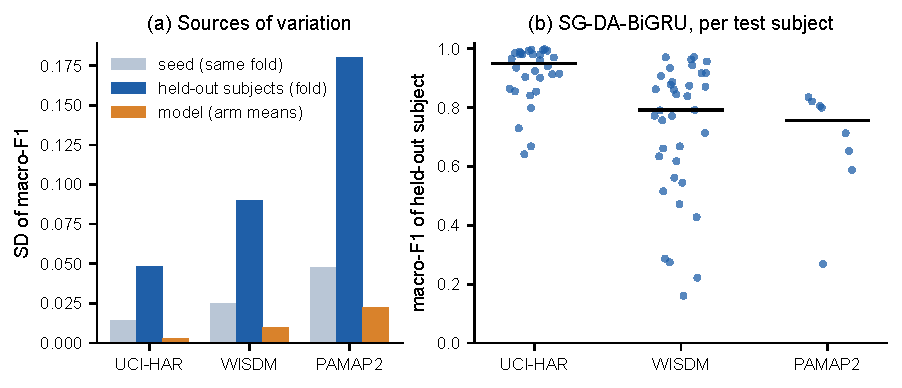
\includegraphics[width=\linewidth]{fig_variance}
  \caption{(a) Standard deviation of macro-F1 across seeds within a fold, across folds (held-out subjects) and across model means. (b) Macro-F1 of SG-DA-BiGRU for each held-out subject (mean over seeds); bars are medians.}
  \label{fig:variance}
\end{figure}

\subsection{Fixed splits give different rankings}
\label{sec:fixed}
Table~\ref{tab:official} reports the fixed train/test splits. On UCI-HAR's official split, CNN+BiGRU leads clearly (0.913 against 0.875--0.884 for every other model), a gap that largely disappears under LOSO (0.925 against 0.916--0.922). On WISDM, Channel-only ranks first on the fixed split and last under LOSO. Rank correlations between fixed-split and LOSO orderings (Figure~\ref{fig:rank}) are weak and not significant: Kendall's $\tau=0.29$ (UCI-HAR), $-0.14$ (WISDM) and $0.43$ (PAMAP2). A claim that one model beats another on one fixed split, even averaged over five seeds, is therefore weak evidence about generalisation to new users.

\begin{table}[!htbp]
\centering
\caption{Fixed train/test split (secondary), macro-F1 mean $\pm$ standard deviation over five seeds. UCI-HAR uses the official split; WISDM and PAMAP2 use a fixed seeded subject-level 80/20 split.}
\label{tab:official}
\small
\begin{tabular}{lccc}
\toprule
Model & UCI-HAR & WISDM & PAMAP2 \\
\midrule
BiGRU & 0.883 $\pm$ 0.008 & 0.824 $\pm$ 0.024 & 0.681 $\pm$ 0.028 \\
BiLSTM+Attn & 0.881 $\pm$ 0.006 & 0.800 $\pm$ 0.014 & 0.667 $\pm$ 0.045 \\
CNN+BiGRU & \textbf{0.913} $\pm$ 0.006 & 0.835 $\pm$ 0.013 & \textbf{0.758} $\pm$ 0.037 \\
DeepConvLSTM & 0.876 $\pm$ 0.014 & 0.833 $\pm$ 0.011 & 0.735 $\pm$ 0.064 \\
\midrule
SG-DA-BiGRU & 0.883 $\pm$ 0.010 & 0.815 $\pm$ 0.030 & 0.666 $\pm$ 0.075 \\
DA-BiGRU & 0.875 $\pm$ 0.005 & 0.830 $\pm$ 0.016 & 0.689 $\pm$ 0.065 \\
Channel-only & 0.878 $\pm$ 0.009 & \textbf{0.838} $\pm$ 0.021 & 0.692 $\pm$ 0.033 \\
Temporal-only & 0.884 $\pm$ 0.003 & 0.805 $\pm$ 0.035 & 0.702 $\pm$ 0.021 \\
\bottomrule
\end{tabular}
\end{table}

\begin{figure}[!htbp]
  \centering
  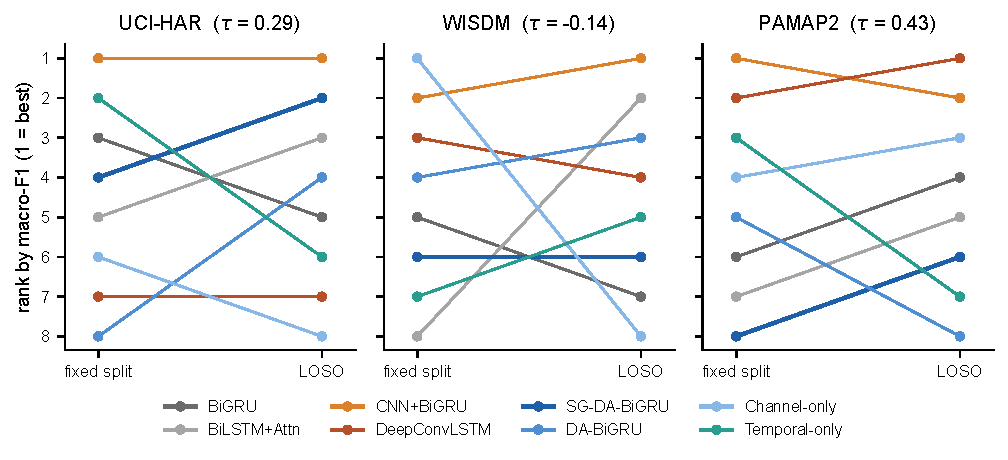
\includegraphics[width=\linewidth]{fig_rankshift}
  \caption{Model ranks (by macro-F1) on the fixed split versus under LOSO. Crossing lines indicate rank changes; $\tau$ is Kendall's rank correlation.}
  \label{fig:rank}
\end{figure}

\subsection{Computational cost}
Table~\ref{tab:eff} and Figure~\ref{fig:eff} relate accuracy to cost. The attention variants add at most 8.4k parameters to the BiGRU (127.8k vs.\ 119.4k on UCI-HAR), and the spectral gate itself adds 33. CNN+BiGRU has about twice as many parameters (259k), but because its pooling layers shorten the sequence fed to the BiGRU, it needs the fewest FLOPs (18.7M per UCI-HAR window, against 28.8M for SG-DA-BiGRU). DeepConvLSTM is the most expensive model by a wide margin (175M FLOPs on UCI-HAR, 435M on PAMAP2). The FLOP count misses the FFT, but measured GPU latency does not. At batch size 32 the two spectral-gated arms take 4.2\,ms on UCI-HAR, against 1.6\,ms for DA-BiGRU, 1.3\,ms for Temporal-only, 1.1\,ms for the plain BiGRU and 2.7\,ms for CNN+BiGRU. On this hardware, the 33-parameter gate therefore makes inference about 2.6 times slower than the same model without it (4.2 vs.\ 1.6\,ms) and buys no accuracy. CPU latencies favour the LSTM models because of PyTorch's optimised LSTM path on CPU, so they reflect library support rather than architectural cost.

\begin{table}[!htbp]
\centering
\caption{Computational cost. Parameters (thousands) and FLOPs (millions per window) per data set; latency (ms per batch) measured on UCI-HAR inputs on an RTX 3050 Laptop GPU (batch 1 and 32) and on one CPU thread (batch 1). FLOPs exclude the FFT.}
\label{tab:eff}
\small
\setlength{\tabcolsep}{4.2pt}
\begin{tabular}{lccccccccc}
\toprule
& \multicolumn{3}{c}{Params (k)} & \multicolumn{3}{c}{MFLOPs / window} & \multicolumn{3}{c}{Latency, UCI-HAR (ms)} \\
\cmidrule(lr){2-4}\cmidrule(lr){5-7}\cmidrule(lr){8-10}
Model & UCI & WISDM & PAMAP2 & UCI & WISDM & PAMAP2 & GPU b1 & GPU b32 & CPU b1 \\
\midrule
BiGRU & 119.4 & 118.3 & 124.8 & 26.6 & 10.5 & 27.8 & 1.02 & 1.06 & 17.90 \\
BiLSTM+Attn & 161.8 & 160.3 & 168.7 & 37.5 & 14.8 & 39.1 & 1.02 & 1.15 & 2.35 \\
CNN+BiGRU & 259.3 & 258.3 & 263.9 & 18.7 & 7.0 & 19.7 & 1.94 & 2.73 & 5.13 \\
DeepConvLSTM & 458.1 & 359.8 & 852.0 & 175.0 & 35.4 & 435.1 & 3.64 & 3.58 & 5.40 \\
\midrule
SG-DA-BiGRU & 127.8 & 126.6 & 133.3 & 28.8 & 11.4 & 29.9 & 4.33 & 4.21 & 18.62 \\
DA-BiGRU & 127.8 & 126.6 & 133.3 & 28.8 & 11.4 & 29.9 & 3.13 & 1.64 & 16.86 \\
Channel-only & 119.5 & 118.3 & 125.0 & 26.6 & 10.5 & 27.8 & 3.49 & 4.25 & 18.24 \\
Temporal-only & 127.8 & 126.6 & 133.1 & 28.8 & 11.4 & 29.9 & 1.62 & 1.27 & 17.50 \\
\bottomrule
\end{tabular}
\end{table}

\begin{figure}[!htbp]
  \centering
  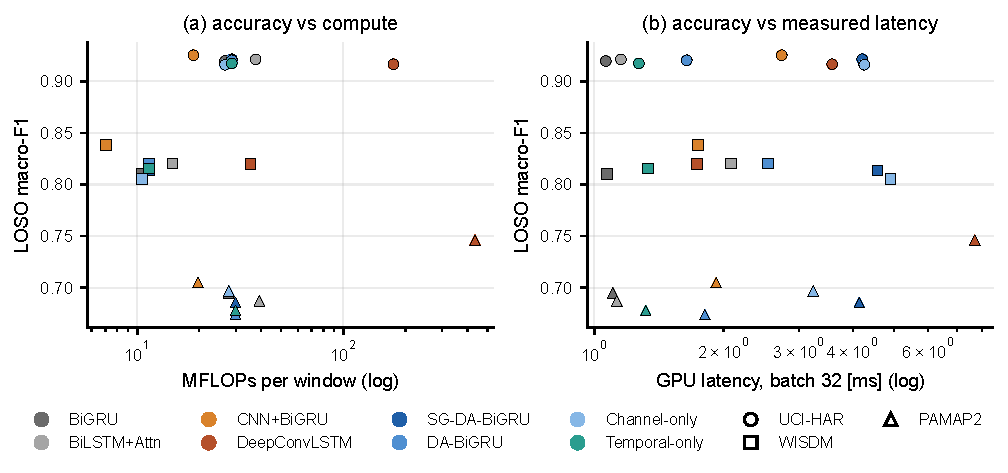
\includegraphics[width=\linewidth]{fig_eff}
  \caption{LOSO macro-F1 against (a) FLOPs per window and (b) measured GPU latency at batch size 32 (log scales). Marker shape encodes the data set.}
  \label{fig:eff}
\end{figure}

\section{Discussion}
\label{sec:discussion}

\paragraph{Why the spectral gate does not help.}
The gate's descriptors do carry activity information. A logistic regression on the $2C$ descriptors alone, with subject-grouped five-fold cross-validation, reaches macro-F1 0.71 on UCI-HAR and 0.51 on WISDM. Figure~\ref{fig:desc} shows what that information is. On accelerometer channels the low-band ratio is near zero for static postures (sitting, standing, lying) and 0.2--0.5 for locomotion. In other words, the descriptors mainly separate static from dynamic activities, which every model already does almost perfectly (Figure~\ref{fig:perclass}). Gyroscope channels have high ratios for every activity and so provide little contrast. The errors that remain are among similar activities, e.g.\ upstairs versus downstairs, sitting versus standing, or household tasks in PAMAP2. These differ in fine temporal structure that a per-channel scalar gain cannot express. In addition, a two-layer BiGRU with z-scored inputs can learn to emphasise or ignore channels through its input weights, so the attention block mostly re-learns something the recurrent layer already provides.

\begin{figure}[!htbp]
  \centering
  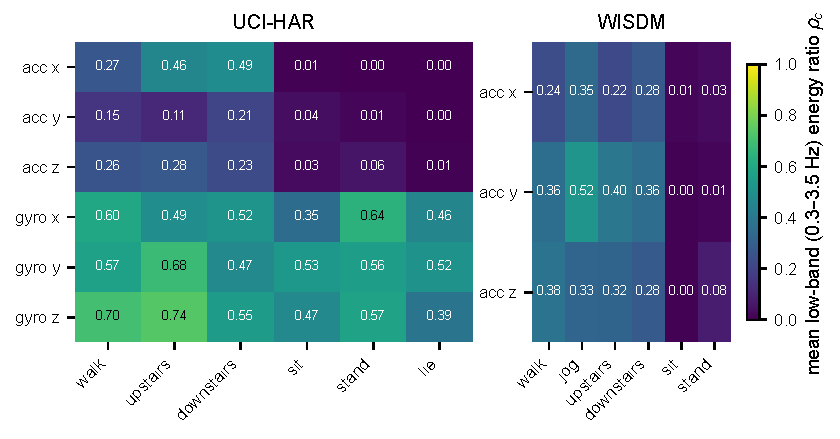
\includegraphics[width=0.9\linewidth]{fig_descriptors}
  \caption{Mean low-band (0.3--3.5\,Hz) energy ratio $\rho_c$ per channel and activity, computed on z-scored windows. On accelerometer axes the descriptor mainly separates static from dynamic activities. PAMAP2 is omitted because its preprocessed windows were not available on the analysis machine.}
  \label{fig:desc}
\end{figure}

\paragraph{Why convolutional front-ends help more.}
Both hybrids learn banks of short temporal filters before any recurrence. These filters are what distinguishes the hard class pairs, and CNN+BiGRU also shortens the sequence the BiGRU must integrate. The advantage is modest (0.016 pooled) and not significant after correction, but it is consistent across data sets in direction and in ranking. This matches earlier findings that convolutional feature extraction is the most reliable ingredient in deep HAR \cite{ordonez2016deep,hammerla2016deep,bock2021improving}.

\paragraph{Relation to reported results.}
Recent dual-attention models report 96--99\% accuracy on these benchmarks \cite{zhang2025dualinaba,he2025tgahar}. Our numbers are lower (e.g.\ 0.92 on UCI-HAR, 0.84 on WISDM) because test subjects are unseen and model selection never touches them; the gap between protocols is expected \cite{gholamiangonabadi2020deep,jordao2018human} and is not evidence of weaker models. The more important difference is methodological. Our results suggest that improvements of one or two points attributed to attention components are within the range that fold composition and seeds alone produce, unless they are shown on many folds with paired tests.

\paragraph{Recommendations.}
From this study we suggest the following for papers proposing HAR architectures:
\begin{enumerate}
  \item Evaluate on unseen subjects, and select checkpoints with subject-wise validation data. On noisy validation sets, select on the target metric (macro-F1) rather than validation loss, and report the distribution of selected epochs.
  \item Use enough folds to make significance attainable (with eight folds the smallest Holm-corrected Wilcoxon $p$ over seven comparisons is 0.055), average seeds within folds, and pool folds across data sets for the primary test.
  \item Compare a new component against the identical model without it, i.e.\ an ablation, not only against weaker or differently tuned baselines.
  \item Report equivalence-aware statistics (Bayesian signed-rank or confidence intervals with a stated practical-equivalence margin) so that null results are informative.
  \item Fix the decision rule before running the final experiment, and report the outcome either way.
  \item Report measured latency alongside FLOPs: here a component with 33 parameters and negligible FLOPs made GPU inference 2.6 times slower.
\end{enumerate}

\section{Limitations and Threats to Validity}
\label{sec:limits}
\emph{Hyper-parameters.} All models share one configuration (except DeepConvLSTM, which uses its published one) and were not individually tuned. Tuning could change individual results, but it would have to favour the attention components systematically to change the conclusion, and nested tuning under LOSO was beyond our compute budget.
\emph{Scope.} We study three widely used benchmarks with 6--18 channels and 2.56\,s windows. Attention may matter more with many sensor positions, longer windows or multimodal inputs \cite{ma2019attnsense}.
\emph{Statistical power.} PAMAP2 has only eight subjects; its per-data-set tests are descriptive, and its fold scores are noisy (one held-out subject scores 0.27).
\emph{Protocol revision.} The protocol was revised once, before the final run and identically for all models, and the first run gave the same answer to the primary question. The Bayesian, Friedman and per-class analyses were not part of the pre-specified rule.
\emph{Metric definition.} Macro-F1 over the union of true and predicted classes penalises predictions of activities a test subject never performed. This lowers absolute PAMAP2 scores but applies to all models.
\emph{Hardware.} Latency was measured on one laptop GPU and one CPU, and the relative cost of the FFT may differ on embedded hardware.
\emph{Descriptor analysis.} Figure~\ref{fig:desc} uses global rather than per-fold normalisation and covers two of the three data sets.

\section{Conclusion}
We set out to propose a spectral-gated dual-attention BiGRU for wearable HAR and evaluated it, together with its ablations and four baselines, under a subject-independent protocol with five seeds per fold, 1{,}320 runs and a decision rule fixed in advance. The spectral gate is practically equivalent to the same model without it ($\Delta=+0.0008$ macro-F1, 99.5\% posterior probability of $|\Delta|<0.01$), and no attention variant improves on a plain BiGRU. Convolutional-recurrent hybrids rank highest, though not significantly after correction. Differences among architectures are dwarfed by differences among held-out subjects, and fixed-split rankings are poor guides to subject-independent ones. For practitioners, a plain BiGRU or a CNN+BiGRU is the better choice on these benchmarks. For researchers, we hope that the protocol, the decision rule and the released per-run results make it easier to test, and if necessary refute, future architectural claims.

\section*{Data and Code Availability}
The three benchmarks are publicly available from their original sources \cite{anguita2013public,kwapisz2011activity,reiss2012introducing}. Code, configurations, the protocol document containing the pre-specified decision rule, all 1{,}320 per-run results, test-set predictions and the scripts that generate every table and figure in this paper are available at [repository URL].

\section*{Declaration of Competing Interest}
The author declares no competing interests.

\section*{Acknowledgements}
[To be completed by the author.]

\section*{Declaration on the Use of Generative AI}
[To be completed by the author according to the target venue's policy.]

\bibliographystyle{unsrtnat}
\bibliography{refs}

\appendix
\section{Supplementary Results}

\begin{table}[h]
\centering
\caption{Subject-independent (LOSO) accuracy, mean $\pm$ standard deviation across folds (each fold averaged over five seeds). Bold marks the best model per column.}
\label{tab:acc}
\small
\begin{tabular}{lcccc}
\toprule
Model & UCI-HAR (10 folds) & WISDM (12) & PAMAP2 (8) & Pooled (30) \\
\midrule
BiGRU & 0.918 $\pm$ 0.049 & 0.840 $\pm$ 0.103 & 0.754 $\pm$ 0.181 & 0.843 $\pm$ 0.130 \\
BiLSTM+Attn & 0.920 $\pm$ 0.049 & 0.841 $\pm$ 0.113 & 0.745 $\pm$ 0.176 & 0.842 $\pm$ 0.133 \\
CNN+BiGRU & \textbf{0.923} $\pm$ 0.042 & \textbf{0.860} $\pm$ 0.102 & 0.764 $\pm$ 0.185 & 0.855 $\pm$ 0.129 \\
DeepConvLSTM & 0.914 $\pm$ 0.051 & 0.845 $\pm$ 0.098 & \textbf{0.801} $\pm$ 0.097 & \textbf{0.856} $\pm$ 0.093 \\
\midrule
SG-DA-BiGRU & 0.920 $\pm$ 0.045 & 0.843 $\pm$ 0.107 & 0.739 $\pm$ 0.183 & 0.841 $\pm$ 0.134 \\
DA-BiGRU & 0.918 $\pm$ 0.047 & 0.846 $\pm$ 0.102 & 0.730 $\pm$ 0.182 & 0.839 $\pm$ 0.135 \\
Channel-only & 0.915 $\pm$ 0.050 & 0.833 $\pm$ 0.107 & 0.757 $\pm$ 0.176 & 0.840 $\pm$ 0.128 \\
Temporal-only & 0.916 $\pm$ 0.053 & 0.843 $\pm$ 0.107 & 0.735 $\pm$ 0.171 & 0.838 $\pm$ 0.131 \\
\bottomrule
\end{tabular}
\end{table}

\end{document}
